\chapter{Power Grid  Security}


On of the implications of the transition from the \acrlong{pg} to the \acrlong{sg}, is the connection of  the traditionally closed and  proprietary energy distribution infrastructure to the Internet. 
Connecting the grid to the Internet  makes the grid available for monitoring and control purposes while exposing the grid to new threats, most notably the threats from external threat actors now able to attack the infrastructure from remote locations. 




\section{Classic Power Grid Security}

The Classical Power Grid consists of systems designed in order to provide a stable supply of electical power to a number of customers. As explained by \citeauthor{knapp2015industrial} in \cite{knapp2015industrial}, \acrshort{ics}s, like the \acrlong{pg}, has traditionally been airgapped systems, not designed with Cyber security in mind, including the continuous software and operating system updates so characteristic of any contemporary computer system. \\

The increased vulnerabilities to external threats observable as a consequence of connecting the grid to the Internet, has resulted in numerous activities related to securing the grid, wile reaping the substantial benefits of keeping the grid online. 



\subsection{Industrial Control System (ICS) Security}


Traditionally, the operational sites of any \acrfull{ics},  has been closed systems, not connected to public networks like the Internet. The \acrshort{pg}, and to some extent\footnote{The \acrshort{scada} subsystem of the \acrlong{sg} is part of the \acrshort{sg} \acrshort{wams} control system} even the \acrshort{sg}, utilises the \acrshort{scada} subsystem, for monitoring and control, 
The principle of "Security by Obscurity" has, as explained by  \citeauthor{humayed2017cyber}  in \cite{humayed2017cyber}, has been a dominant design principle for the traditional, offline, \acrlong{ics}.
As further explained  in \cite{humayed2017cyber}, most attacks on Industrial Control Systems, has been internal prior to 2001. Consequently, over the years following 2001, most of the attacks on \acrshort{ics} has been of external origin.





\subsection{Cyber Physical Systems security}

A \acrfull{cps} constitutes, as described in the previous chapter, of a physical production system, typically a \acrfull{ics} combined with a Cyber system connected the production system to public networks for monitoring and management purposes. As described by \citeauthor{humayed2017cyber} in \cite{humayed2017cyber}, the \acrshort{cps} may be of several types, amongst them the \acrshort{sg}.

The \acrshort{cps} constitutes a highly complex system,  combining physical production systems with systems connecting the physical systems to the outside world.\  

The authors of \cite{humayed2017cyber} provides some general characteristics of \acrshort{cps} security threats common to the various types of \acrshort{cps} identified:



\begin{itemize}
    \item 
    \item  
\end{itemize}




In addition, \figureautorefname{ }  \ref{fig:CP-Vulnerabilities-SG.png} presents vulnerabilities chrarcteristic of \acrshort{sg} \acrshort{ics}s:


\begin{figure}[ht]
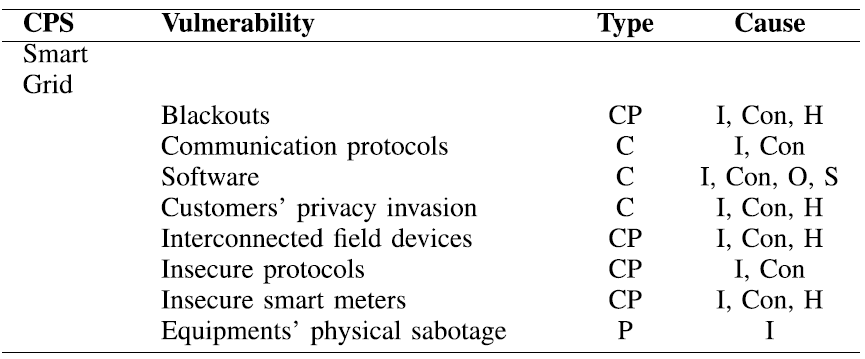
\includegraphics[width=\linewidth]{figures/CP-Vulnerabilities-SG.png}
\caption[\acrlong{cps} vulnerabilities for the \acrlong{sg}]{\acrlong{cps} vulnerabilities for the \acrlong{sg}, with causes. \cite[p. 1809]{humayed2017cyber}}
\label{fig:CP-Vulnerabilities-SG.png}
\end{figure}

As described in \citeauthor{humayed2017cyber}, "Type" and "Cause" are abbreviated as follows: Type classifications (C:CYBER, CP: CYBER-PHYSICAL, P: PHYSICAL, I: ISOLATION) and Causes (Con: CONNECTIVITY, O: OPENNESS, H: HETEROGENEITY,  S: MANY STAKEHOLDERS).






\section{Smart Grid  Security} 

\subsection{Smart Grid Security Requirements}
In order to protect the grid form new threat scenarios, a set of new security requirements needs to be defined in order to address the new situation. 
 
In \cite{Shapsough2015}, \citeauthor{Shapsough2015}  describes some information security concepts related to \acrlong{sg} security, defining the requirements in order to ensure the information security of the \acrshort{sg}. Thus, the \acrlong{sg} information security requirements might be summarised as follows:

\begin{itemize}
    \item \textbf{Availability} of the \acrlong{sg} is mandatory, as a violation of \acrlong{sg} availability implies a disruption of electricity. The immediate recovery from the lack of availability, is critical to the continued operation of a large number of services in a modern society.  
    \item \textbf{Integrity} violations in the \acrshort{sg} might affect power management, due to unauthorised modifications by illegitimate users. 
    \item \textbf{Confidentiality} violations will affect the privacy of users. Asides from the annoyance of privacy violations, power grid usage information might be indicative of empty buildings which could be a nice target for thieves. \item \textbf{Authentication} violations enables unauthorised access to private information, as well as \acrfull{sg} resources.
    \item \textbf{Authorisation} implements access control, preventing improper access to and management of \acrshort{sg} resources by unauthorised individuals.      \item \textbf{Non-Repudiation} violations enables individuals to deny being accessing or utilising \acrshort{sg} resources. Being able to track down actions of individual actors accessing \acrshort{sg} is vital due to the criticality of the \acrshort{sg}.
\end{itemize}


\section{Smart Grid Network Reliability and Security}

Two interrelated concepts are essential for the safe operation of the \acrshort{sg}:  
\begin{itemize}
    \item \acrlong{sg} \textbf{Network Reliability } which is important for the correct \acrshort{sg} operation, minimising the risk of \acrshort{sg} operational failures caused by \textbf{unintentional disruptive events} affecting \acrshort{sg} operations.
    
    \item \acrlong{sg} \textbf{Network Security}  which is important for the correct \acrshort{sg} operation, minimising the risk of \acrshort{sg} operational failures caused by \textbf{intentional malicious events}  affecting \acrshort{sg} operations.
\end{itemize}



\subsection{Smart Grid Network Reliability}

\subsection{Smart Grid Network Security}




    

\subsection{Synchrophasor  Protocol Threats}
Given the criticality of Time Synchronisation for the correct operation of the \acrshort{sg}, it is of vital importance to be aware of which threats imposes security risks related to the underlying Time Protocol. As explained by \citeauthor{mizrahi2014security} in \Cite{mizrahi2014security}, several attacker types could inflict a number of attacks on various time protocols. My introductory coverage of time protocol threats includes descriptions on attacker types and attack types, for reference purposes.







